% !TeX program = xelatex
\documentclass{article}
\usepackage{kotex}
\usepackage[a4paper,left=3cm, right=3cm, top=2cm, bottom=2cm]{geometry}
\usepackage{amsmath}
\usepackage{graphicx}
\usepackage{caption}
\usepackage{setspace}
\usepackage{xcolor}
\usepackage{titlesec}
\usepackage{amssymb}
\usepackage{tcolorbox}
\usepackage{wrapfig}
\usepackage{amsthm}
\usepackage{multirow}
\usepackage{array}
\usepackage{tikz}
\usepackage{longtable}
\usepackage{pgfplots}
\pgfplotsset{compat=1.18}

\title{1.8 Introduction to Linear Transformations}
\date{}
\author{}
\setstretch{1.3}

\titleformat{name=\section, numberless}
  {\normalfont\large\bfseries\color{blue}}
  {}
  {0pt}
  {}
\geometry{a4paper, margin=1in}

\newcommand{\redheading}[1]{{\vspace{2mm}\noindent\Large\bfseries\color{red!55!black} #1\par}\vspace{2mm}}

\newtheoremstyle{mystyle}
  {}{}{\itshape}{}{\bfseries}{.}{.5em}{}
\theoremstyle{mystyle}

\begin{document}
\maketitle

{\itshape\color{blue!45!black}
Up to now matrices have been viewed as rectangular arrays of numbers. In this section we view matrices in a completely different way: as \emph{transformations} that map vectors from one space to another via multiplication. This viewpoint is the foundation for much of our subsequent work.\par}

\redheading{Vectors in $R^n$}

The set of all ordered $n$-tuples of reals is denoted $R^n$; its elements are called \textbf{vectors} and may be written in \emph{comma-delimited form} $(s_1,s_2,\ldots,s_n)$ or, equivalently, as a \emph{column vector}
\[
\mathbf{x}=\begin{bmatrix}x_1\\x_2\\\vdots\\x_n\end{bmatrix}
\]
The \textbf{standard basis vectors} for $R^n$ are
\[
\mathbf{e}_1=\begin{bmatrix}1\\0\\\vdots\\0\end{bmatrix},\quad
\mathbf{e}_2=\begin{bmatrix}0\\1\\\vdots\\0\end{bmatrix},\quad\ldots,\quad
\mathbf{e}_n=\begin{bmatrix}0\\0\\\vdots\\1\end{bmatrix}
\]
Every $\mathbf{x}\in R^n$ can be expressed uniquely as $\mathbf{x}=x_1\mathbf{e}_1+x_2\mathbf{e}_2+\cdots+x_n\mathbf{e}_n$.

\begin{tcolorbox}[colback=teal!4, colframe=teal!65!black, title=Definition 1, fonttitle=\bfseries, boxrule=0.5mm, arc=3mm]
If $T$ is a function with domain $R^n$ and codomain $R^m$, then $T$ is a \textbf{transformation} from $R^n$ to $R^m$, written $T:R^n\to R^m$. In the special case $m=n$, $T$ is called an \textbf{operator} on $R^n$.
\end{tcolorbox}

\redheading{Matrix Transformations}

A linear system with $m$ equations in $n$ unknowns can be written in matrix notation as $\mathbf{w}=A\mathbf{x}$. Viewing multiplication by $A$ as a function that maps $\mathbf{x}\in R^n$ to $\mathbf{w}\in R^m$ gives a \textbf{matrix transformation} (or \textbf{matrix operator} if $m=n$):
\[
T_A:R^n\to R^m,\qquad T_A(\mathbf{x})=A\mathbf{x}
\]
equivalently written $\mathbf{x}\xrightarrow{T_A}\mathbf{w}$.

\subsection*{EXAMPLE 1 | A Matrix Transformation from $R^4$ to $R^3$}
The transformation defined by
\[
w_1=2x_1-3x_2+x_3-5x_4,\quad
w_2=4x_1+x_2-2x_3+x_4,\quad
w_3=5x_1-x_2+4x_3
\]
has standard matrix $A=\begin{bmatrix}2&-3&1&-5\\4&1&-2&1\\5&-1&4&0\end{bmatrix}$. For $\mathbf{x}=\begin{bmatrix}1&-3&0&2\end{bmatrix}^T$,
\[
T_A(\mathbf{x})=A\mathbf{x}=\begin{bmatrix}2&-3&1&-5\\4&1&-2&1\\5&-1&4&0\end{bmatrix}\begin{bmatrix}1\\-3\\0\\2\end{bmatrix}=\begin{bmatrix}1\\3\\8\end{bmatrix}
\]

\subsection*{EXAMPLE 2 | Zero Transformations}
If $0$ is the $m\times n$ zero matrix, then $T_0(\mathbf{x})=0\mathbf{x}=\mathbf{0}$, mapping every vector in $R^n$ to $\mathbf{0}\in R^m$. $T_0$ is the \textbf{zero transformation} from $R^n$ to $R^m$.

\subsection*{EXAMPLE 3 | Identity Operators}
If $I$ is the $n\times n$ identity matrix, then $T_I(\mathbf{x})=I\mathbf{x}=\mathbf{x}$, mapping every vector to itself. $T_I$ is the \textbf{identity operator} on $R^n$.

\redheading{Properties of Matrix Transformations}

\begin{tcolorbox}[colback=red!4, colframe=red!60!black, title=Theorem 1.8.1, boxrule=0.5mm, arc=3mm]
For every matrix $A$, the transformation $T_A:R^n\to R^m$ satisfies, for all $\mathbf{u},\mathbf{v}\in R^n$ and every scalar $k$:\\
(a) $T_A(\mathbf{0})=\mathbf{0}$\qquad
(b) $T_A(k\mathbf{u})=kT_A(\mathbf{u})$\quad\textbf{[Homogeneity]}\\
(c) $T_A(\mathbf{u}+\mathbf{v})=T_A(\mathbf{u})+T_A(\mathbf{v})$\quad\textbf{[Additivity]}\\
(d) $T_A(\mathbf{u}-\mathbf{v})=T_A(\mathbf{u})-T_A(\mathbf{v})$
\end{tcolorbox}
\textbf{Proof.} All four parts are restatements of matrix arithmetic properties from Theorem 1.4.1. $\blacksquare$

It follows from (b) and (c) that matrix transformations preserve linear combinations:
\[
T_A(k_1\mathbf{u}_1+k_2\mathbf{u}_2+\cdots+k_r\mathbf{u}_r)=k_1T_A(\mathbf{u}_1)+k_2T_A(\mathbf{u}_2)+\cdots+k_rT_A(\mathbf{u}_r) \tag{10}
\]

Not every transformation $T:R^n\to R^m$ is a matrix transformation. The following theorem answers both when $T$ is a matrix transformation, and how to find the associated matrix.

\begin{tcolorbox}[colback=red!4, colframe=red!60!black, title=Theorem 1.8.2, boxrule=0.5mm, arc=3mm]
$T:R^n\to R^m$ is a matrix transformation if and only if for all $\mathbf{u},\mathbf{v}\in R^n$ and every scalar $k$:
\begin{itemize}\setlength\itemsep{0pt}
\item[(i)] $T(\mathbf{u}+\mathbf{v})=T(\mathbf{u})+T(\mathbf{v})$ \quad\textbf{[Additivity]}
\item[(ii)] $T(k\mathbf{u})=kT(\mathbf{u})$ \quad\textbf{[Homogeneity]}
\end{itemize}
\end{tcolorbox}
\textbf{Proof.} ($\Rightarrow$) Follows from Theorem 1.8.1(b)(c). ($\Leftarrow$) Assume (i) and (ii). Using (10) and $\mathbf{x}=x_1\mathbf{e}_1+\cdots+x_n\mathbf{e}_n$,
\[
T(\mathbf{x})=x_1T(\mathbf{e}_1)+\cdots+x_nT(\mathbf{e}_n)=A\mathbf{x},\quad A=[T(\mathbf{e}_1)\mid T(\mathbf{e}_2)\mid\cdots\mid T(\mathbf{e}_n)] \tag{13}
\]
so $T=T_A$. $\blacksquare$

The two properties in Theorem 1.8.2 are called \textbf{linearity conditions}; a transformation satisfying them is called a \textbf{linear transformation}. Thus:

\begin{tcolorbox}[colback=red!4, colframe=red!60!black, title=Theorem 1.8.3, boxrule=0.5mm, arc=3mm]
Every linear transformation from $R^n$ to $R^m$ is a matrix transformation, and conversely every matrix transformation is a linear transformation.
\end{tcolorbox}

\begin{tcolorbox}[colback=red!4, colframe=red!60!black, title=Theorem 1.8.4, boxrule=0.5mm, arc=3mm]
If $T_A:R^n\to R^m$ and $T_B:R^n\to R^m$ satisfy $T_A(\mathbf{x})=T_B(\mathbf{x})$ for every $\mathbf{x}\in R^n$, then $A=B$.
\end{tcolorbox}
\textbf{Proof.} In particular $A\mathbf{e}_j=B\mathbf{e}_j$ for $j=1,\ldots,n$, which means the $j$th columns of $A$ and $B$ are equal for all $j$, so $A=B$. $\blacksquare$

Theorem 1.8.4 establishes a one-to-one correspondence between $m\times n$ matrices and matrix transformations $R^n\to R^m$; we call $A$ the \textbf{standard matrix} for the transformation.

\redheading{Finding the Standard Matrix}

From (13), the standard matrix is
\[
A=[T(\mathbf{e}_1)\mid T(\mathbf{e}_2)\mid\cdots\mid T(\mathbf{e}_n)] \tag{15}
\]

\begin{tcolorbox}[colback=blue!5, colframe=blue!60!black, boxrule=0.5mm, arc=3mm]
\textbf{Procedure for Finding the Standard Matrix}\\
\textbf{Step 1.} Find the images $T(\mathbf{e}_1), T(\mathbf{e}_2),\ldots,T(\mathbf{e}_n)$ of the standard basis vectors for $R^n$.\\
\textbf{Step 2.} Form $A$ with these images as successive columns.
\end{tcolorbox}

\subsection*{EXAMPLE 4 | Finding a Standard Matrix}
Find the standard matrix for $T:R^2\to R^3$ defined by
$T\!\left(\begin{bmatrix}x_1\\x_2\end{bmatrix}\right)=\begin{bmatrix}2x_1+x_2\\x_1-3x_2\\-x_1+x_2\end{bmatrix}$.

\textbf{SOLUTION:} $T(\mathbf{e}_1)=T\!\left(\begin{bmatrix}1\\0\end{bmatrix}\right)=\begin{bmatrix}2\\1\\-1\end{bmatrix}$, $\;T(\mathbf{e}_2)=T\!\left(\begin{bmatrix}0\\1\end{bmatrix}\right)=\begin{bmatrix}1\\-3\\1\end{bmatrix}$. Thus
$A=[T(\mathbf{e}_1)\mid T(\mathbf{e}_2)]=\begin{bmatrix}2&1\\1&-3\\-1&1\end{bmatrix}$.

\subsection*{EXAMPLE 5 | Computing with Standard Matrices}
Using $A$ from Example 4, $T\!\left(\begin{bmatrix}1\\4\end{bmatrix}\right)=\begin{bmatrix}2&1\\1&-3\\-1&1\end{bmatrix}\begin{bmatrix}1\\4\end{bmatrix}=\begin{bmatrix}6\\-11\\3\end{bmatrix}$.

\subsection*{EXAMPLE 6 | Finding a Standard Matrix}
Rewrite $T(x_1,x_2)=(3x_1+x_2,\,2x_1-4x_2)$ in column-vector form and find the standard matrix:
\[
T\!\left(\begin{bmatrix}x_1\\x_2\end{bmatrix}\right)=\begin{bmatrix}3x_1+x_2\\2x_1-4x_2\end{bmatrix}=\begin{bmatrix}3&1\\2&-4\end{bmatrix}\begin{bmatrix}x_1\\x_2\end{bmatrix}
\]
The standard matrix is $\begin{bmatrix}3&1\\2&-4\end{bmatrix}$.

\subsection*{EXAMPLE 7 | Finding a Standard Matrix from Non-Standard Data}
Find the standard matrix $A$ for $T:R^2\to R^2$ given
$T\!\left(\begin{bmatrix}-1\\1\end{bmatrix}\right)=\begin{bmatrix}-5\\5\end{bmatrix}$,\;
$T\!\left(\begin{bmatrix}2\\-1\end{bmatrix}\right)=\begin{bmatrix}7\\-6\end{bmatrix}$.

\textbf{SOLUTION:} Express $\mathbf{e}_1$ and $\mathbf{e}_2$ as linear combinations of the given input vectors:
\[
\begin{bmatrix}1\\0\end{bmatrix}=1\cdot\begin{bmatrix}-1\\1\end{bmatrix}+1\cdot\begin{bmatrix}2\\-1\end{bmatrix},\qquad
\begin{bmatrix}0\\1\end{bmatrix}=2\cdot\begin{bmatrix}-1\\1\end{bmatrix}+1\cdot\begin{bmatrix}2\\-1\end{bmatrix}
\]
Using linearity:
\[
T(\mathbf{e}_1)=\begin{bmatrix}-5\\5\end{bmatrix}+\begin{bmatrix}7\\-6\end{bmatrix}=\begin{bmatrix}2\\-1\end{bmatrix},\qquad
T(\mathbf{e}_2)=2\begin{bmatrix}-5\\5\end{bmatrix}+\begin{bmatrix}7\\-6\end{bmatrix}=\begin{bmatrix}-3\\4\end{bmatrix}
\]
Thus $A=\begin{bmatrix}2&-3\\-1&4\end{bmatrix}$.

\redheading{Reflection Operators}

Reflections about coordinate axes (in $R^2$) or planes (in $R^3$) through the origin are matrix transformations. In each case the standard matrix is obtained by finding the images of $\mathbf{e}_1,\ldots,\mathbf{e}_n$ and using Formula (15).

\vspace{3mm}
\noindent\textbf{Table 1.} Reflection operators on $R^2$.
\renewcommand{\arraystretch}{1.6}
\begin{center}
\begin{tabular}{|l|l|c|}
\hline
\textbf{Operator} & \textbf{Images of $\mathbf{e}_1,\mathbf{e}_2$} & \textbf{Standard Matrix} \\
\hline
Reflection about $x$-axis: $T(x,y)=(x,-y)$ & $(1,0),\;(0,-1)$ & $\begin{bmatrix}1&0\\0&-1\end{bmatrix}$ \\
\hline
Reflection about $y$-axis: $T(x,y)=(-x,y)$ & $(-1,0),\;(0,1)$ & $\begin{bmatrix}-1&0\\0&1\end{bmatrix}$ \\
\hline
Reflection about $y=x$: $T(x,y)=(y,x)$ & $(0,1),\;(1,0)$ & $\begin{bmatrix}0&1\\1&0\end{bmatrix}$ \\
\hline
\end{tabular}
\end{center}

\vspace{3mm}
\noindent\textbf{Table 2.} Reflection operators on $R^3$.
\begin{center}
\begin{tabular}{|l|l|c|}
\hline
\textbf{Operator} & \textbf{Images of $\mathbf{e}_1,\mathbf{e}_2,\mathbf{e}_3$} & \textbf{Standard Matrix} \\
\hline
Refl.\ about $xy$-plane: $T(x,y,z)=(x,y,-z)$ & $(1,0,0),(0,1,0),(0,0,-1)$ & $\begin{bmatrix}1&0&0\\0&1&0\\0&0&-1\end{bmatrix}$ \\
\hline
Refl.\ about $xz$-plane: $T(x,y,z)=(x,-y,z)$ & $(1,0,0),(0,-1,0),(0,0,1)$ & $\begin{bmatrix}1&0&0\\0&-1&0\\0&0&1\end{bmatrix}$ \\
\hline
Refl.\ about $yz$-plane: $T(x,y,z)=(-x,y,z)$ & $(-1,0,0),(0,1,0),(0,0,1)$ & $\begin{bmatrix}-1&0&0\\0&1&0\\0&0&1\end{bmatrix}$ \\
\hline
\end{tabular}
\end{center}
\renewcommand{\arraystretch}{1}

\redheading{Projection Operators}

Orthogonal projections onto coordinate axes or planes are also matrix transformations.

\vspace{3mm}
\noindent\textbf{Table 3.} Orthogonal projection operators on $R^2$.
\renewcommand{\arraystretch}{1.5}
\begin{center}
\begin{tabular}{|l|l|c|}
\hline
\textbf{Operator} & \textbf{Images of $\mathbf{e}_1,\mathbf{e}_2$} & \textbf{Standard Matrix} \\
\hline
Projection onto $x$-axis: $T(x,y)=(x,0)$ & $(1,0),\;(0,0)$ & $\begin{bmatrix}1&0\\0&0\end{bmatrix}$ \\
\hline
Projection onto $y$-axis: $T(x,y)=(0,y)$ & $(0,0),\;(0,1)$ & $\begin{bmatrix}0&0\\0&1\end{bmatrix}$ \\
\hline
\end{tabular}
\end{center}

\vspace{3mm}
\noindent\textbf{Table 4.} Orthogonal projection operators on $R^3$.
\begin{center}
\begin{tabular}{|l|l|c|}
\hline
\textbf{Operator} & \textbf{Images of $\mathbf{e}_1,\mathbf{e}_2,\mathbf{e}_3$} & \textbf{Standard Matrix} \\
\hline
Proj.\ onto $xy$-plane: $T(x,y,z)=(x,y,0)$ & $(1,0,0),(0,1,0),(0,0,0)$ & $\begin{bmatrix}1&0&0\\0&1&0\\0&0&0\end{bmatrix}$ \\
\hline
Proj.\ onto $xz$-plane: $T(x,y,z)=(x,0,z)$ & $(1,0,0),(0,0,0),(0,0,1)$ & $\begin{bmatrix}1&0&0\\0&0&0\\0&0&1\end{bmatrix}$ \\
\hline
Proj.\ onto $yz$-plane: $T(x,y,z)=(0,y,z)$ & $(0,0,0),(0,1,0),(0,0,1)$ & $\begin{bmatrix}0&0&0\\0&1&0\\0&0&1\end{bmatrix}$ \\
\hline
\end{tabular}
\end{center}
\renewcommand{\arraystretch}{1}

\redheading{Rotation Operators}

A \textbf{rotation operator} on $R^2$ rotates vectors counterclockwise about the origin through angle $\theta$. The standard basis vectors map to $T(\mathbf{e}_1)=(\cos\theta,\sin\theta)$ and $T(\mathbf{e}_2)=(-\sin\theta,\cos\theta)$, giving the \textbf{rotation matrix}:
\[
R_\theta=\begin{bmatrix}\cos\theta&-\sin\theta\\\sin\theta&\cos\theta\end{bmatrix} \tag{19}
\]
The clockwise rotation matrix is $R_{-\theta}=\begin{bmatrix}\cos\theta&\sin\theta\\-\sin\theta&\cos\theta\end{bmatrix}$.

\begin{center}
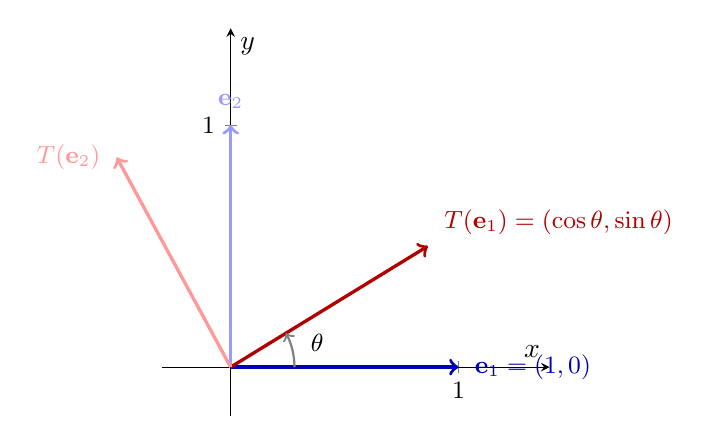
\begin{tikzpicture}
\begin{axis}[
  width=6.5cm, height=6.5cm,
  axis lines=center,
  xmin=-0.3, xmax=1.4, ymin=-0.2, ymax=1.4,
  xtick={1}, ytick={1},
  xlabel={$x$}, ylabel={$y$},
  tick label style={font=\small},
  clip=false]
\addplot[->, thick, blue!70!black, line width=1.2pt] coordinates {(0,0)(1,0)}
  node[right, xshift=2pt]{\small $\mathbf{e}_1=(1,0)$};
\addplot[->, thick, red!70!black, line width=1.2pt] coordinates {(0,0)(0.866,0.5)}
  node[above right, xshift=2pt]{\small $T(\mathbf{e}_1)=(\cos\theta,\sin\theta)$};
\addplot[->, thick, blue!40, line width=1.2pt] coordinates {(0,0)(0,1)}
  node[above, yshift=2pt]{\small $\mathbf{e}_2$};
\addplot[->, thick, red!40, line width=1.2pt] coordinates {(0,0)(-0.5,0.866)}
  node[left, xshift=-2pt]{\small $T(\mathbf{e}_2)$};
\draw[->, gray, line width=0.8pt] (0.28,0) arc[start angle=0, end angle=30, radius=0.28];
\node at (0.38,0.1) {\small $\theta$};
\end{axis}
\end{tikzpicture}
\end{center}

\vspace{2mm}
\noindent\textbf{Table 5.} Rotation operator on $R^2$.
\renewcommand{\arraystretch}{1.5}
\begin{center}
\begin{tabular}{|l|l|c|}
\hline
\textbf{Operator} & \textbf{Images of $\mathbf{e}_1,\mathbf{e}_2$} & \textbf{Standard Matrix} \\
\hline
CCW rotation by $\theta$ about origin & $(\cos\theta,\sin\theta),\;(-\sin\theta,\cos\theta)$ & $\begin{bmatrix}\cos\theta&-\sin\theta\\\sin\theta&\cos\theta\end{bmatrix}$ \\
\hline
\end{tabular}
\end{center}
\renewcommand{\arraystretch}{1}

\subsection*{EXAMPLE 8 | A Rotation Matrix}
Find the image of $\mathbf{x}=(1,1)$ under a rotation of $\theta=\pi/6$ ($=30°$) about the origin.

\textbf{SOLUTION:} From (19):
\[
R_{\pi/6}\begin{bmatrix}1\\1\end{bmatrix}
=\begin{bmatrix}\cos(\pi/6)&-\sin(\pi/6)\\\sin(\pi/6)&\cos(\pi/6)\end{bmatrix}\begin{bmatrix}1\\1\end{bmatrix}
=\begin{bmatrix}\dfrac{\sqrt{3}}{2}&-\dfrac{1}{2}\\[6pt]\dfrac{1}{2}&\dfrac{\sqrt{3}}{2}\end{bmatrix}\begin{bmatrix}1\\1\end{bmatrix}
=\begin{bmatrix}\dfrac{\sqrt{3}-1}{2}\\[6pt]\dfrac{1+\sqrt{3}}{2}\end{bmatrix}\approx\begin{bmatrix}0.37\\1.37\end{bmatrix}
\]
In comma-delimited notation, $R_{\pi/6}(1,1)\approx(0.37,1.37)$.

\noindent\textbf{Remark.} Rotations in $R^3$ are substantially more complicated and will be considered later.

\section*{Exercise Set 1.8}
\begin{enumerate}
\item[1.] Find the domain and codomain of $T_A(\mathbf{x})=A\mathbf{x}$ when:\\
(a) $A$ has size $3\times2$.\quad (b) $A$ has size $2\times3$.\quad (c) $A$ has size $3\times3$.\quad (d) $A$ has size $1\times6$.

\item[3.] Find the domain and codomain of the transformation defined by the equations.\\
(a) $w_1=4x_1+5x_2$,\; $w_2=x_1-8x_2$\\
(b) $w_1=5x_1-7x_2$,\; $w_2=6x_1+x_2$,\; $w_3=2x_1+3x_2$

\item[5.] Find the domain and codomain of $T$ defined by the matrix product.\\
(a) $\begin{bmatrix}3&1&2\\6&7&1\end{bmatrix}\begin{bmatrix}x_1\\x_2\\x_3\end{bmatrix}$\qquad
(b) $\begin{bmatrix}2&-1\\4&3\\2&-5\end{bmatrix}\begin{bmatrix}x_1\\x_2\end{bmatrix}$

\item[7.] Find the domain and codomain of $T$ defined by the formula.\\
(a) $T(x_1,x_2)=(2x_1-x_2,\,x_1+x_2)$\quad
(b) $T(x_1,x_2,x_3)=(4x_1+x_2,\,x_1+x_2)$

\item[9.] Find the domain and codomain.
\[
T\!\left(\begin{bmatrix}x_1\\x_2\end{bmatrix}\right)=\begin{bmatrix}4x_1\\x_1-x_2\\3x_2\end{bmatrix}
\]

\item[11.] Find the standard matrix for the transformation defined by the equations.\\
(a) $w_1=2x_1-3x_2+x_3$,\; $w_2=3x_1+5x_2-x_3$\\
(b) $w_1=7x_1+2x_2-8x_3$,\; $w_2=-x_2+5x_3$,\; $w_3=4x_1+7x_2-x_3$

\item[13.] Find the standard matrix for $T$ defined by the formula.\\
(a) $T(x_1,x_2)=(x_2,\,-x_1,\,x_1+3x_2,\,x_1-x_2)$\\
(b) $T(x_1,x_2,x_3,x_4)=(7x_1+2x_2-x_3+x_4,\;x_2+x_3,\;-x_1)$

\item[14.] Find the standard matrix for the operator $T$ defined by the formula.\\
(a) $T(x_1,x_2)=(2x_1-x_2,\,x_1+x_2)$\quad
(d) $T(x_1,x_2,x_3)=(4x_1,\,7x_2,\,-8x_3)$

\item[15.] Find the standard matrix for the operator $T:R^3\to R^3$ defined by
\[
w_1=3x_1+5x_2-x_3,\quad w_2=4x_1-x_2+x_3,\quad w_3=3x_1+2x_2-x_3
\]
and compute $T(-1,2,4)$ by direct substitution and by matrix multiplication.

\item[17.] Find the standard matrix for $T$ and use it to compute $T(\mathbf{x})$.\\
(a) $T(x_1,x_2)=(-x_1+x_2,\,x_2)$;\; $\mathbf{x}=(-1,4)$\\
(b) $T(x_1,x_2,x_3)=(2x_1-x_2+x_3,\,x_2+x_3,\,0)$;\; $\mathbf{x}=(2,1,-3)$

\item[19.] Find $T_A(\mathbf{x})$ and express your answer in matrix form.\\
(a) $A=\begin{bmatrix}1&2\\3&4\end{bmatrix}$;\; $\mathbf{x}=\begin{bmatrix}3\\-2\end{bmatrix}$\qquad
(b) $A=\begin{bmatrix}-1&2&0\\3&1&5\end{bmatrix}$;\; $\mathbf{x}=\begin{bmatrix}-1\\1\\3\end{bmatrix}$

\item[21.] Use Theorem 1.8.2 to show that $T$ is a matrix transformation.\\
(a) $T(x,y)=(2x+y,\,x-y)$\quad
(b) $T(x_1,x_2,x_3)=(x_1+x_3,\,x_1+x_2)$

\item[23.] Use Theorem 1.8.2 to show that $T$ is \emph{not} a matrix transformation.\\
(a) $T(x,y)=(x^2,\,y)$\quad
(b) $T(x,y,z)=(x,\,y,\,xz)$

\item[25.] A function of the form $f(x)=mx+b$ is commonly called a ``linear function'' because its graph is a line. Is $f$ a matrix transformation on $R$? Explain.

\item[27.] The images of the standard basis vectors for $R^3$ under a linear transformation $T:R^3\to R^3$ are given. Find the standard matrix for $T$ and compute $T(\mathbf{x})$.
\[
T(\mathbf{e}_1)=\begin{bmatrix}1\\3\\0\end{bmatrix},\quad
T(\mathbf{e}_2)=\begin{bmatrix}0\\0\\1\end{bmatrix},\quad
T(\mathbf{e}_3)=\begin{bmatrix}4\\-3\\-1\end{bmatrix};\qquad
\mathbf{x}=\begin{bmatrix}2\\1\\0\end{bmatrix}
\]

\item[29.] Use matrix multiplication to find the reflection of $(-1,2)$ about the\\
(a) $x$-axis.\quad (b) $y$-axis.\quad (c) line $y=x$.

\item[31.] Use matrix multiplication to find the reflection of $(2,-5,3)$ about the\\
(a) $xy$-plane.\quad (b) $xz$-plane.\quad (c) $yz$-plane.

\item[33.] Use matrix multiplication to find the orthogonal projection of $(2,-5)$ onto the\\
(a) $x$-axis.\quad (b) $y$-axis.

\item[37.] Use matrix multiplication to find the image of $(3,-4)$ when rotated about the origin through angle\\
(a) $\theta=30°$.\quad (b) $\theta=-60°$.\quad (c) $\theta=45°$.

\item[39.] Let $T:R^2\to R^2$ be a linear operator for which the images of the standard basis vectors are $T(\mathbf{e}_1)=(a,b)$ and $T(\mathbf{e}_2)=(c,d)$. Find $T(1,1)$.

\item[44.] If multiplication by $A$ rotates a vector $\mathbf{x}$ in the $xy$-plane through angle $\theta$, what is the effect of multiplying $\mathbf{x}$ by $A^T$? Explain your reasoning.

\item[45.] Find the standard matrix $A$ for the linear transformation $T:R^2\to R^2$ for which
\[
T\!\left(\begin{bmatrix}1\\1\end{bmatrix}\right)=\begin{bmatrix}-1\\-2\end{bmatrix},\qquad
T\!\left(\begin{bmatrix}2\\3\end{bmatrix}\right)=\begin{bmatrix}-2\\5\end{bmatrix}
\]

\item[50.] \textbf{(a)} Prove: If $T:R^n\to R^m$ is a matrix transformation, then $T(\mathbf{0})=\mathbf{0}$.\\
\textbf{(b)} Find an example of a mapping $T:R^n\to R^m$ for which $T(\mathbf{0})=\mathbf{0}$ but $T$ is not a matrix transformation.
\end{enumerate}

\end{document}
